\section{Auswertung}
\label{sec:Auswertung}
\subsection{Messung der Molwärme}

Die Molwärme $C_V$ bei konstantem Volumen experimentell zu bestimmen,
gestaltet sich aufgrund der dadurch auftretenden hohen Drücke schwierig.
Daher wird zuerst $C_p$ bei konstantem Druck bestimmt 
und anschließend wird durch den Zusammenhang in Gleichung \refeq{eq:korrekt} $C_V$ bestimmt.
Mit der zugeführten Energeie
\begin{equation*}
    E = U\cdot I \cdot \Delta t,
\end{equation*}
lässt sich die volumenabhängige Molwärme $C_p$ bestimmen
\begin{equation*}
    C_p = \frac{M}{m} \cdot \frac{E}{\Delta T}.
\end{equation*}
Dabei bezeichnet $U$ die gemessene Spannung,
$I$ die Stromstärke, 
$\Delta t$ das Zeitintervall zwischen zwei Messungen,
$\Delta T$ den Temperaturunterschied,
$M$ die molare Masse der Probe und
$m$ die Probenmasse.
Die  Werte sind in Tabelle \eqref{tab:Messwerte} dargestelt.
\begin{table}[ht]
    \centering
    \caption{Die aufgenommene Wärmemenge und $C_V$ berechnet mit den Messwerten für Strom,Spannung, Zeit und Temperatur.}
    \begin{tabular}{rrrrrr}
    \toprule
    U/V & I/mA & $\Delta t$/s & $\Delta T$ K & E/J & $C_p$  \\ 
    \midrule
    16   & 150  & 0   & 0   & 0   & 0    \\
    15.85& 151.3& 321 & 10.1& 771 & 14.1 \\
    15.99& 152.3& 353 & 10.2& 848 & 15.5 \\
    16.07& 152.9& 406 & 10  & 989 & 18.3 \\
    16.13& 153.3& 388 & 10  & 953 & 17.6 \\
    16.17& 153.5& 410 & 9.8 & 1014& 19.0 \\
    16.21& 153.8& 459 & 10.1& 1050& 20.9 \\ 
    16.24& 153.9& 421 & 9.7 & 1108& 20.0 \\
    16.26& 154.1& 443 & 10  & 1181& 20.5 \\
    16.28& 154.2& 471 & 10  & 1186& 21.8 \\
    16.29& 154.3& 472 & 9.8 & 1382& 22.4 \\
    16.30& 154.4& 550 & 10.1& 1047& 25.3 \\
    16.31& 154.5& 416 & 9.9 & 1094& 19.6 \\
    16.32& 154.5& 434 & 9.9 & 1346& 20.3 \\
    16.32& 154.5& 534 & 10  & 1055& 25   \\
    16.32& 154.6& 418 & 10  & 1027& 19.5 \\
    16.32& 154.7& 407 & 9.8 & 1243& 19.4 \\
    16.32& 154.6& 492 & 9.8 & 2687& 23.3 \\
    16.32& 154.7& 1065& 9.9 & 199 & 50.2 \\
    16.32& 154.6& 79  & 10.2& 1071& 3.6  \\
    16.31& 154.7& 424 & 10.2& 1309& 19.4 \\
    16.31& 154.7& 519 & 9.8 & 358 & 24.8 \\
    16.31& 154.8& 142 & 10.1& 1123& 6.5  \\
    \bottomrule
    \end{tabular}
    \label{tab:Messwerte}
\end{table}

Mit dem linearen Ausdehnungskoeffizienten $\alpha$ aus \cite*{sample} wird $C_V$ berechnet.
Die Werte für den temperaturabhängigen Ausdehnungskoeffizienten sind samt ihrem Fit durch linearer Regression in Abbildung \refeq{fig:alpha} dargestellt.
\begin{figure}[h] 
  \centering
     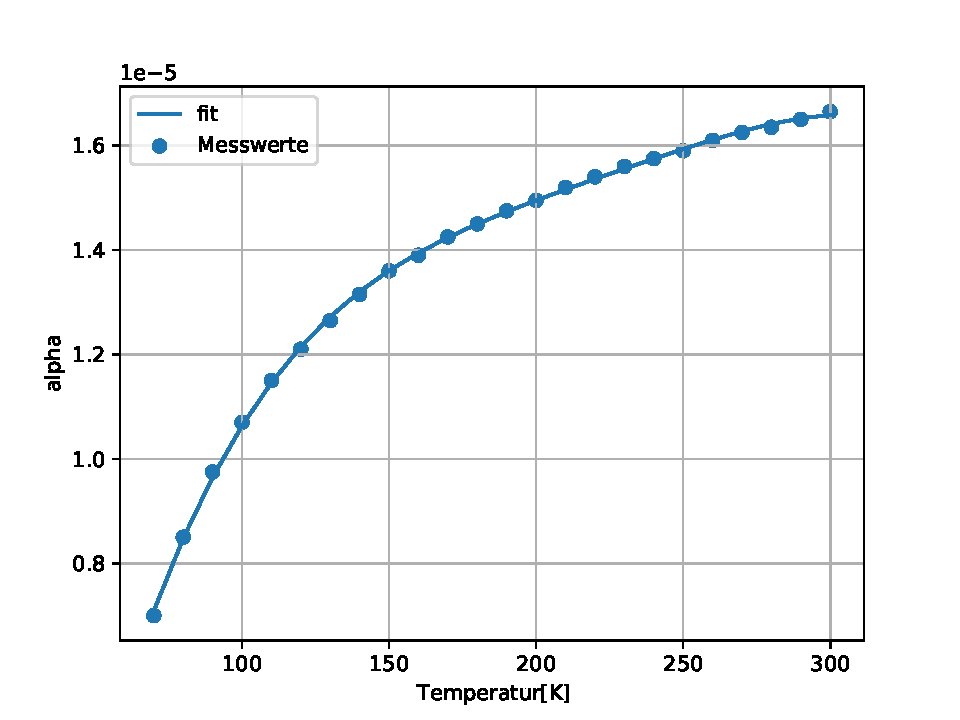
\includegraphics[width=0.7\textwidth]{Auswertung/Plots/alpha.pdf}
  \caption{Werte des temperaturabhängigen Ausdehnungskoeffizienten mit zugehörigem Fit.}
  \label{fig:alpha}
\end{figure}
Daraus ergibt sich mit der Korrekturformel \refeq{eq:korrekt}, die in Abbildung \ref{fig:C_v} dargestellte Temperaturabhängigkeit der Molwärme.
\begin{figure}[h] 
    \centering
       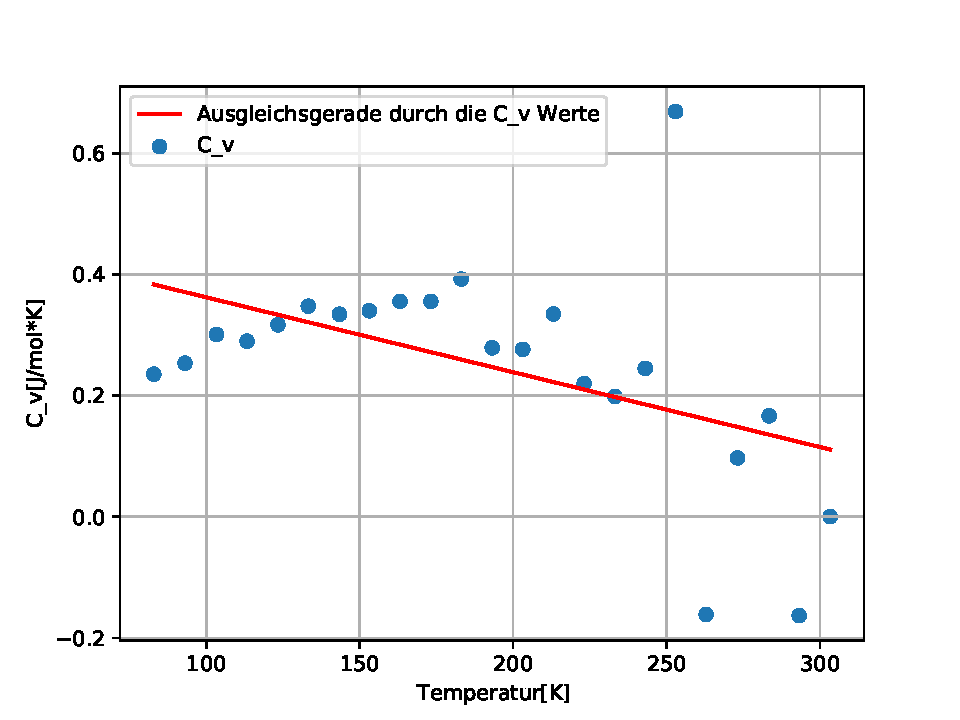
\includegraphics[width=0.7\textwidth]{Auswertung/Plots/C_v.pdf}
    \caption{Berechnete Werte der temperaturabhängigen Molwärme.}
    \label{fig:C_v}
\end{figure}



\subsection{Bestimmung der Debye-Temperatur}
Um die Debye-Temperatur $\theta_D$ zu bestimmen wird die Tabelle \ref{tab:debey} verwendet werden.
\begin{figure}[h] 
    \centering
       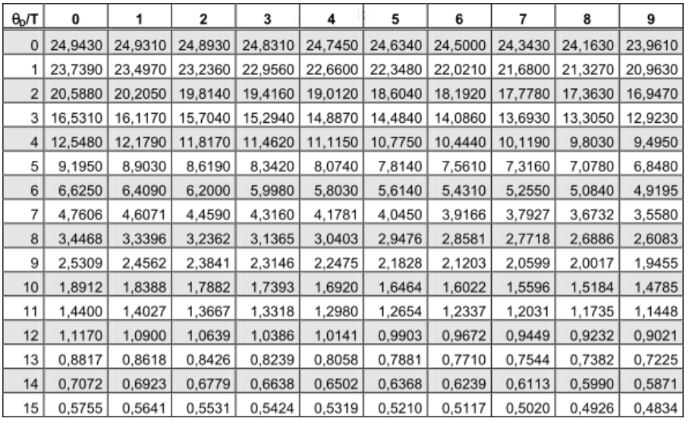
\includegraphics[width=0.8\textwidth]{Tabellen/debey.JPG}
    \caption{Werte der Debye-Funktion.\cite{sample}}
    \label{tab:debey}
\end{figure}
Diese sind in Tabelle \ref{tab:debey2} dargestellt.
\begin{table}[ht]
    \centering
    \caption{Die aufgenommene Wärmemenge und $C_V$ berechnet mit den Messwerten für Strom, Spannung, Zeit und Temperatur.}
    \begin{tabular}{rrrr}
    \toprule
    T/K & $C_V$ & $\frac{\theta_D}{T}$ & $\theta_D$  \\ 
    \midrule
    82.9 & 14.1& 3.6& 298.4 \\ 
    93   & 15.4& 3.3& 306.9 \\
    103.3& 18.3& 2.6& 268.5 \\
    113.3& 17.6& 2.7& 305.9 \\
    123.4& 19  & 2.4& 296.1 \\
    133.2& 20.8& 1.9& 253   \\
    143.4& 20.0& 2.1& 301.1 \\
    153.1& 20.5& 2.0& 306.2 \\
    163.1& 21.8& 1.7& 277.2 \\
    173.2& 22.3& 1.5& 259.8 \\
    183.0& 25.3& 0  & 0     \\ 
    193.2& 19.5& 2.3& 444.3 \\
    203.1& 20.3& 2.1& 426.5 \\
    213.1& 24.9& 0  & 0     \\ 
    223.1& 19.3& 2.3& 513.1 \\
    233.2& 19.2& 2.4& 559.6 \\
    243  & 23.2& 1.2& 291.6 \\
    252.9& 50  & 0  & 0     \\ 
    262.9& 3.4 & 8.0& 2103.2 \\
    173.1& 19.1& 2.4& 415.44 \\
    283.4& 24.6& 0.5& 151.7 \\
    293.2& 6.32& 6.2& 1817.84 \\
    \bottomrule
    \end{tabular}
    \label{tab:debey2}
\end{table}
Es ergibt sich ein Mittelwert von
\begin{equation*}
    \frac{\theta_D}{T}\cdot T =  443.08 K \; .
\end{equation*}

Aus der Forderung 
\begin{equation}
    \int_0^{\omega_\text D} Z(\omega) d\omega = 3 N_\text L
\end{equation}
kann die Debye-Temperatur für ein gegebenes Material auch bestimmt werden. Dazu wird das Integral über die Verteilungsfunktion 
\begin{equation}
    Z(\omega)d\omega = \frac{L^3}{2\pi^2}\omega^2\left(\frac{1}{v_\text{l}^3}+\frac{2}{v_{\text{t}}^3}\right)d\omega
\end{equation}
ausgeführt:
\begin{align*}
	\int_0^{\omega_D} \frac{L^3}{2\pi^2}\omega^2\left(\frac{1}{v_\text{l}^3}+\frac{2}{v_\text{tr}^3}\right) d\omega &\overset{!}{=} 3 N_L\\
	\frac{L^3}{6\pi^2}\omega_D^3\left(\frac{1}{v_\text{l}^3}+\frac{2}{v_\text{tr}^3}\right)  &= 3N_L\\
	\left[\frac{18\pi^2N_L}{L^3}\left(\frac{1}{v_\text{l}^3}+\frac{2}{v_\text{tr}^3}\right)^{-1} \right]^{\frac{1}{3}} &= \omega_D \,\text.
\end{align*}
Die Größe $L$ ist die Länge der Probe, welche nicht gegeben ist. Diese kann aber mittels einer Umrechnung der Loschmidtschen Zahl $N_L$ eliminiert werden. Es ergibt sich:
\begin{align*}
	L^3 = V &= \frac{m}{\rho_\text{Cu}}\qquad N_L = N_A\frac{m}{M}\\
	\Rightarrow \frac{N_L}{L^3} &= N_A\frac{\rho_\text{Cu}}{M}\,\text.
\end{align*}
Dabei ist $N_A$ die Avogadokonstante.
Mit den Werten $m = \SI{342}{\gram}$, $v_\text{l} = \SI{4.7}{\kilo\metre\per\second}$ und $v_\text{tr} = \SI{2.26}{\kilo\meter\per\second}$ kann über
\begin{equation*}
	\theta_D = \frac{\hbar\omega_D}{k_\text{B}}= \frac{\hbar}{k_\text{B}}\left[\frac{18\pi^2\rho_\text{Cu} N_A}{M}\left(\frac{1}{v_\text{l}^3}+\frac{2}{v_\text{tr}^3}\right)^{-1} \right]^{\frac{1}{3}} = \SI{331.991}{\kelvin}
\end{equation*} bestimmt werden. Dabei sind $k_B$ die Boltzmannkonstante und $\hbar$ das reduzierte Plancksche Wirkungsquantum.

